\documentclass[border=6pt,tikz]{standalone}
\usepackage{tikz}
\usepackage{amsmath,amssymb}
\usetikzlibrary{arrows.meta,positioning,fit,backgrounds,calc,shapes.geometric,decorations.pathreplacing,patterns}
\definecolor{ink}{HTML}{1B2430}
\definecolor{muted}{HTML}{6B7785}
\definecolor{accent}{HTML}{2F6FB5}
\definecolor{accent2}{HTML}{C1611F}
\definecolor{good}{HTML}{2E7D5B}
\definecolor{soft}{HTML}{EDF2F7}
\definecolor{soft2}{HTML}{FBEDE2}
\definecolor{soft3}{HTML}{E6F0E9}
\tikzset{
  box/.style={draw=ink,line width=.7pt,rounded corners=2pt,fill=soft,inner sep=4pt,align=center,font=\sffamily\small},
  boxa/.style={box,fill=soft2},
  boxb/.style={box,fill=soft3},
  plain/.style={align=center,font=\sffamily\small,text=ink},
  tiny/.style={align=center,font=\sffamily\scriptsize,text=muted},
  ar/.style={-{Stealth[length=2.4mm]},draw=ink,line width=.7pt},
  arm/.style={-{Stealth[length=2.4mm]},draw=muted,line width=.6pt,dashed},
  nd/.style={circle,draw=ink,line width=.7pt,fill=white,minimum size=7mm,inner sep=0pt,font=\sffamily\scriptsize},
  ndf/.style={nd,fill=soft},
  ndt/.style={nd,fill=soft2},
}

\begin{document}
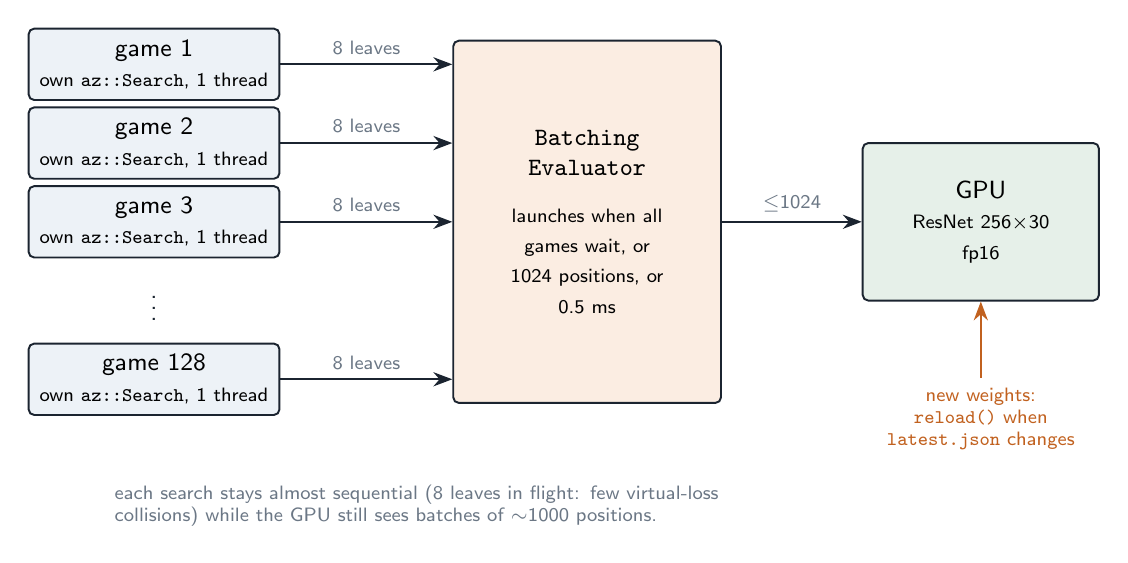
\begin{tikzpicture}[x=1mm,y=1mm]
  \foreach \i/\lbl in {0/game 1,1/game 2,2/game 3,4/game 128} {
    \node[box,minimum width=30mm] (g\i) at (0,-\i*10) {\lbl\\\scriptsize own \texttt{az::Search}, 1 thread};
  }
  \node[plain] at (0,-30) {$\vdots$};
  \node[boxa,minimum width=34mm,minimum height=46mm] (b) at (55,-20)
    {\texttt{Batching}\\\texttt{Evaluator}\\[2mm]\scriptsize launches when all\\\scriptsize games wait, or\\\scriptsize 1024 positions, or\\\scriptsize 0.5 ms};
  \node[boxb,minimum width=30mm,minimum height=20mm] (gpu) at (105,-20) {GPU\\\scriptsize ResNet 256$\times$30\\\scriptsize fp16};
  \foreach \i in {0,1,2,4} { \draw[ar] (g\i.east) -- node[tiny,above,sloped]{8 leaves} (b.west |- g\i.east); }
  \draw[ar] (b.east) -- node[tiny,above]{$\le$1024} (gpu.west);
  \node[tiny,text=accent2,align=center] (rl) at (105,-45) {new weights:\\\texttt{reload()} when\\\texttt{latest.json} changes};
  \draw[ar,draw=accent2] (rl.north) -- (gpu.south);
  \node[tiny,text width=110mm,align=left] at (50,-56)
   {each search stays almost sequential (8 leaves in flight: few virtual-loss\\collisions) while the GPU still sees batches of $\sim$1000 positions.};
\end{tikzpicture}
\end{document}
